\documentclass[DIN, pagenumber=false, fontsize=11pt, parskip=half]{scrartcl}

\usepackage{amsmath}
\usepackage{amsfonts}
\usepackage{amssymb}
\usepackage{enumitem}
\usepackage[utf8]{inputenc} 
\usepackage[ngerman]{babel} 
\usepackage[T1]{fontenc} 
\usepackage{pgfplots}
\usepackage{xcolor}
\usepackage{listings}
\usepackage{float}
\usepackage{graphicx}

\definecolor{mygreen}{RGB}{28,172,0} % color values Red, Green, Blue
\definecolor{mylilas}{RGB}{170,55,241}

\lstset{language=Matlab,%
    %basicstyle=\color{red},
    breaklines=true,%
    morekeywords={matlab2tikz},
    keywordstyle=\color{blue},%
    morekeywords=[2]{1}, keywordstyle=[2]{\color{black}},
    identifierstyle=\color{black},%
    stringstyle=\color{mylilas},
    commentstyle=\color{mygreen},%
    showstringspaces=false,%without this there will be a symbol in the places where there is a space
    numbers=left,%
    numberstyle={\tiny \color{black}},% size of the numbers
    numbersep=9pt, % this defines how far the numbers are from the text
    emph=[1]{for,end,break},emphstyle=[1]\color{red}, %some words to emphasise
    %emph=[2]{word1,word2}, emphstyle=[2]{style},    
}

\title{Einführung in die Neuroinformatik}
\author{Tim Luchterhand, Paul Nykiel}

\begin{document}
    \maketitle
    \section{Aufgabe}
    \subsection{DGL}
    \begin{equation*}
        \tau \dot{u}_j(t) = -u_j(t) + \sum_{i=1}^n c_{ij} \cdot y_i(t-d_{ij}) + x_j(t)
    \end{equation*}
    Erstes Neuron:
    \begin{equation*}
        \tau \dot{u}_1(t) = -u_1(t) + x_1(t)
    \end{equation*}
    Zweites Neuron:
    \begin{equation*}
        \tau \dot{u}_2(t) = -u_2(t) + 0.8 u_1(t) 
    \end{equation*}
    \subsection{Verlauf}
    \begin{tikzpicture}
        \begin{axis}[ 
            xlabel=$t$,
            ylabel={$y_i(t)$},
            xmin=0,
            xmax=30,
            ymin=0,
            ymax=1,
            width=\textwidth,
            height=5cm,
            thick,
        ] 
            \addplot [domain=0:15, color=blue, samples=1000]{1-e^(5-x)};
            \addplot [domain=15:30, color=blue, samples=1000, forget plot]{e^(15-x)};
            \addlegendentry{$y_1(t)$}
            \addplot [domain=0:15, color=green, samples=1000]{0.8*(1-e^(5-x))};
            \addplot [domain=15:30, color=green, samples=1000, forget plot]{0.8*(e^(15-x))};
            \addlegendentry{$y_2(t)$}
        \end{axis}
    \end{tikzpicture} 
    \subsection{Maximum} %TODO Mehr Text
    Erstes Neuron: $\max(y_1(t)) = 1$, da der maximale Eingangswert $\max(x_1(t)) = 1$ und das Neuron keine Energie erzeugt. 
    Zweites Neuron: $\max(y_2(t)) = 0.8$, da der maximale Eingangswert $\max(u_1(t)) = 0.8$ und das Neuron keine Energie erzeugt. 

    \subsection{Matlab}
    \begin{enumerate}[label=(\alph*)]
        \item Matlab Code:
            \lstinputlisting{b01a01.m}
        
        \item Plots:
            \begin{figure}[H]
                \centering
                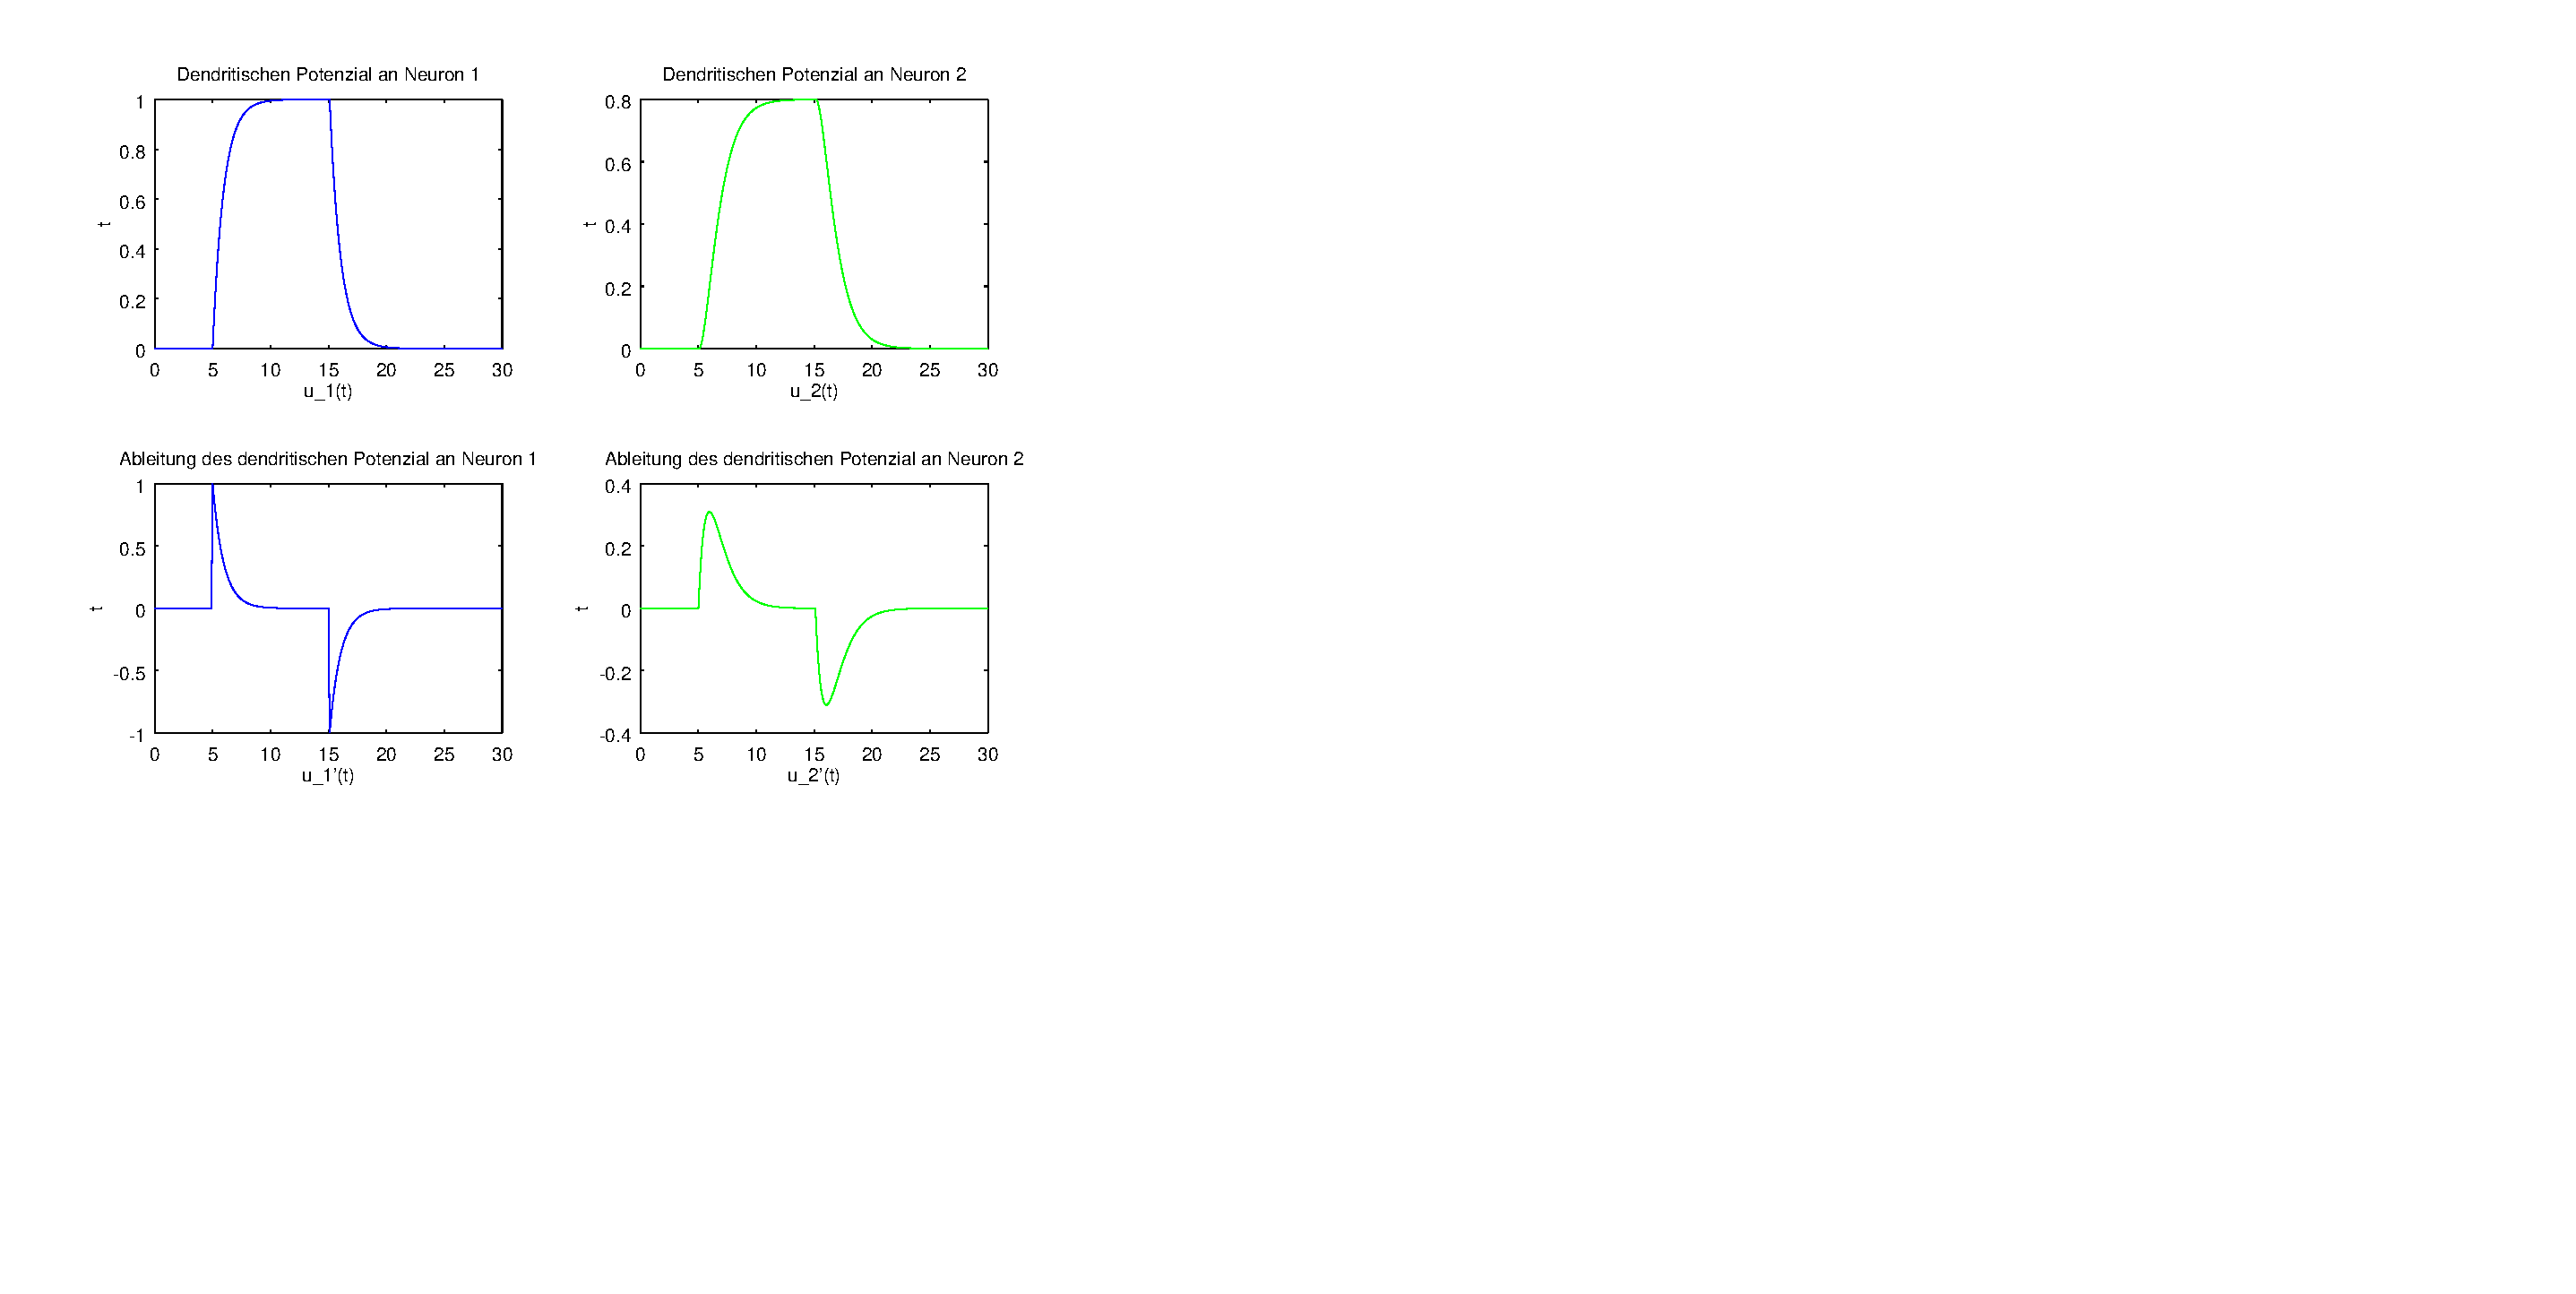
\includegraphics[trim = {0 9cm 27cm 0}, clip,width=\textwidth]{Plot}
                \caption{Dendritischen Potentiale und deren jeweilige Ableitungen}
            \end{figure} 

        \item Ab $t=15$ fallen die Funktionswerte wieder ab, so dass sie für $t \to \infty$ wieder bei $0$ sind...%TODO Mehr Text
    \end{enumerate}

    \subsection{Zeitkonstante}
    \begin{enumerate}[label=(\alph*)]
        \item Mit steigender Zeitkonstante nimmt die Flankensteigung am Ausgang ab, das Neuron reagiert langsamer.
            Bei geringerer Zeitkonstante reagiert das Neuron schneller. %TODO Bilder
            \begin{figure}[H]
                \centering
                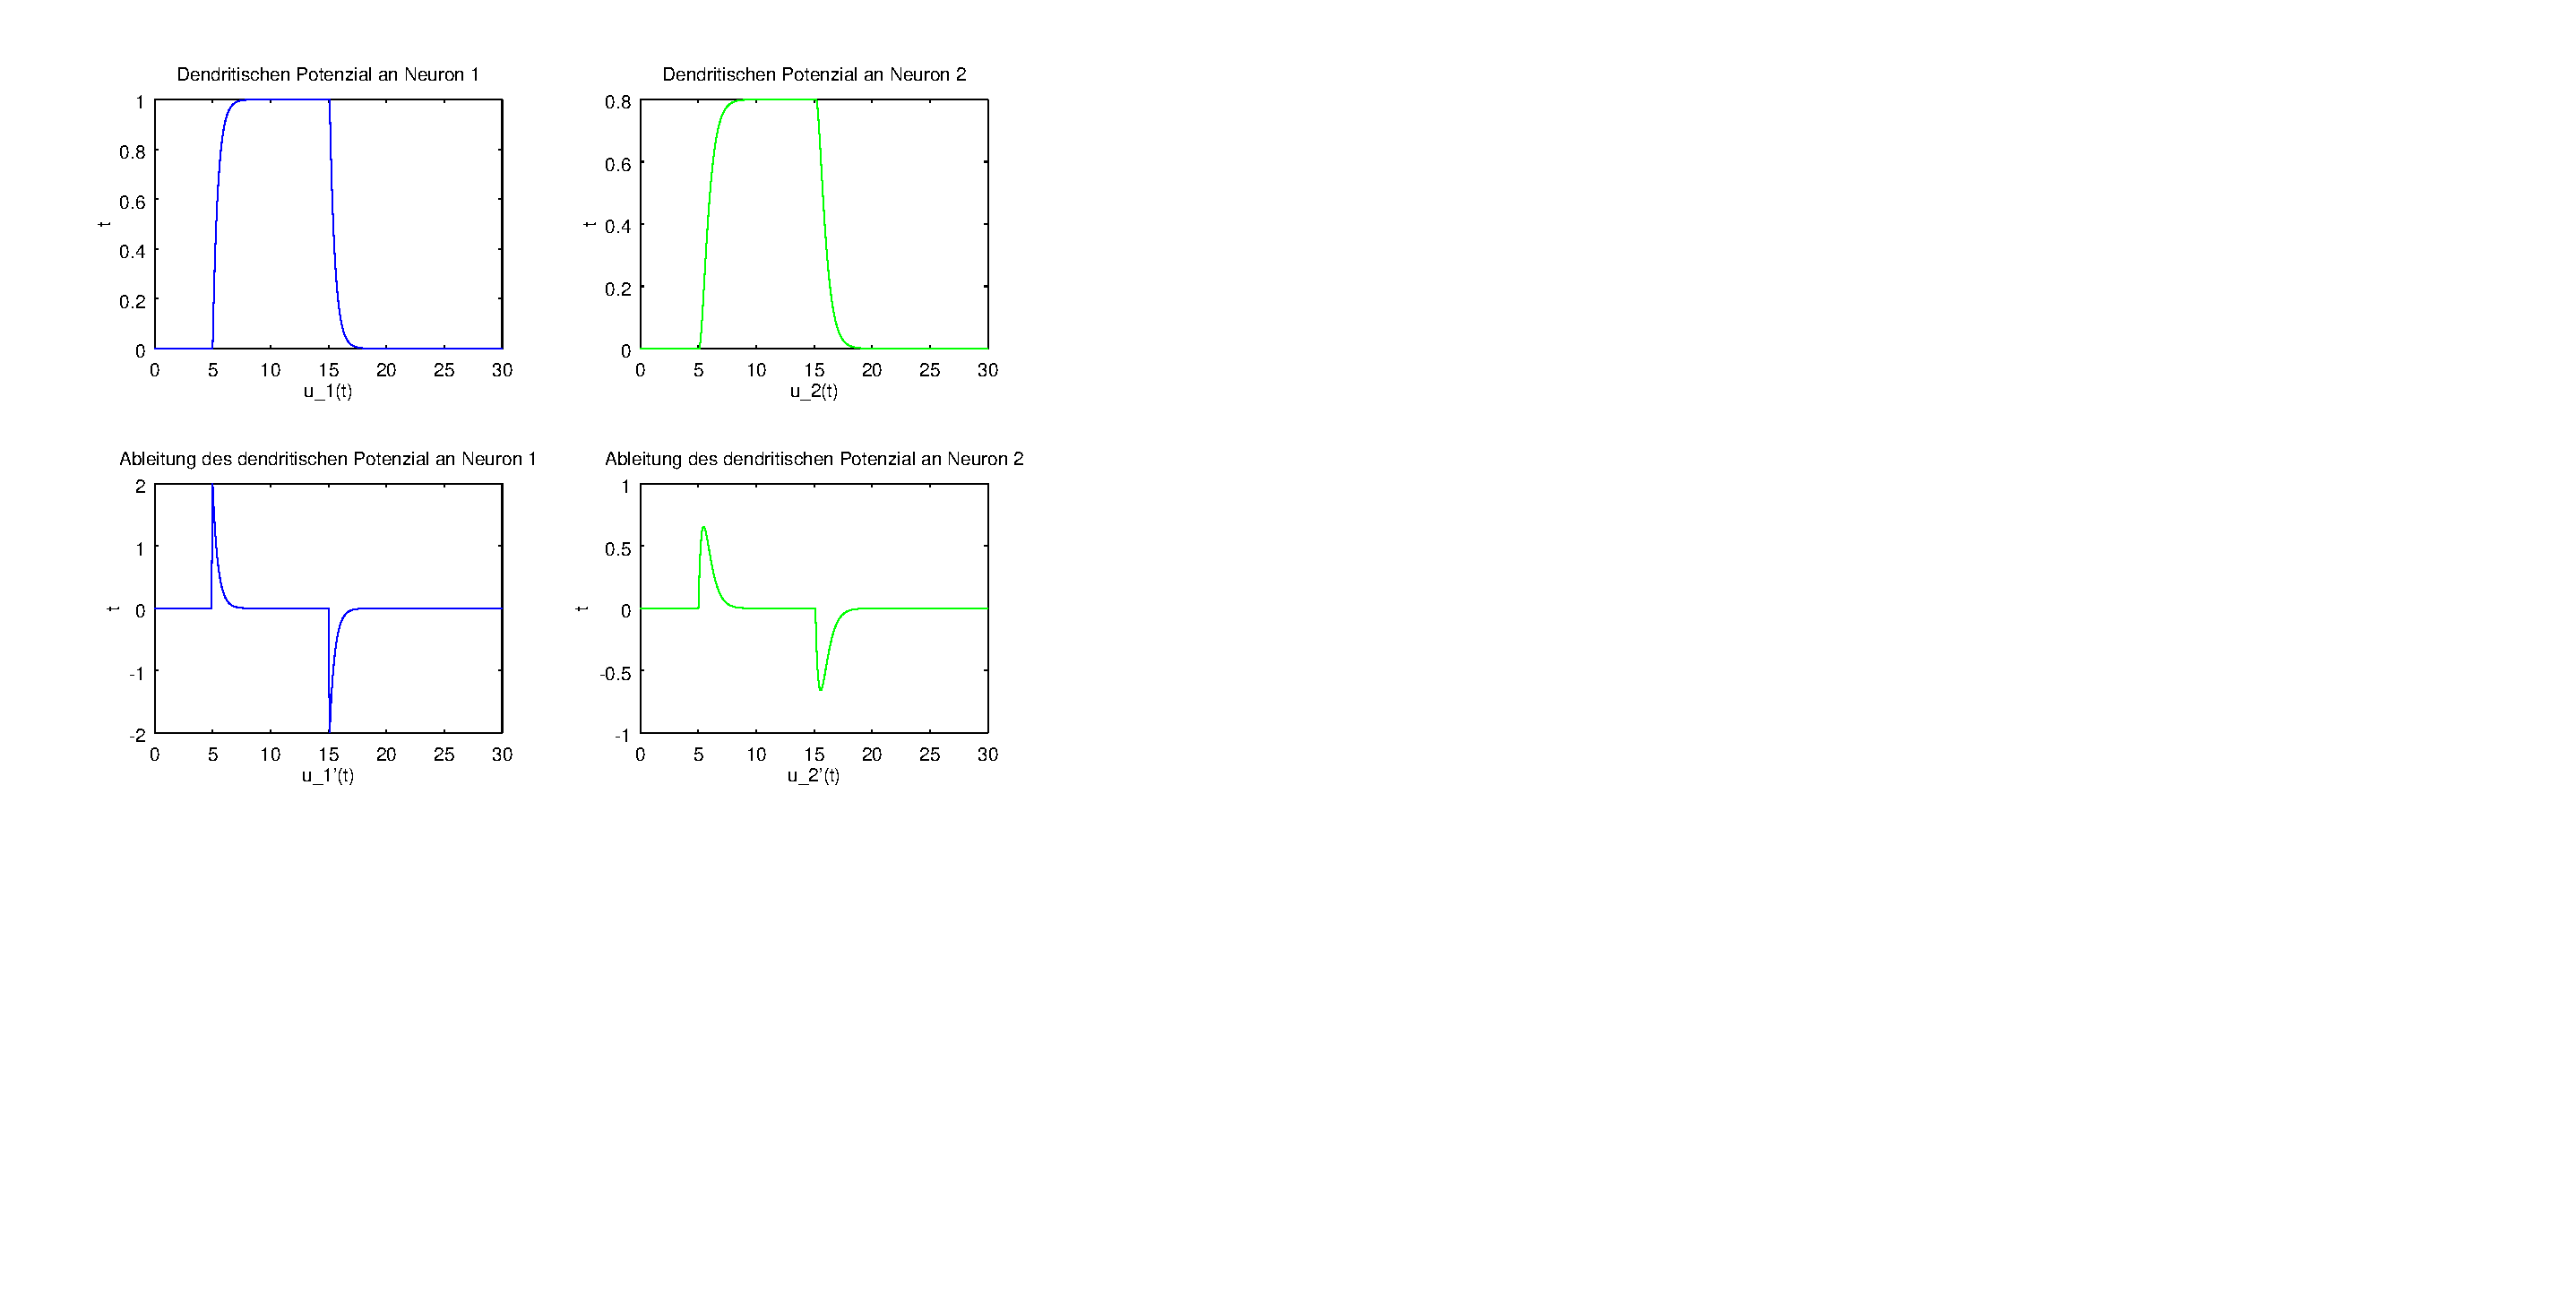
\includegraphics[trim = {0 9cm 27cm 0}, clip,width=\textwidth]{Plot_tau05}
                \caption{Dendritischen Potentiale und deren jeweilige Ableitungen mit $\tau=0.5$}
            \end{figure} 
            \begin{figure}[H]
                \centering
                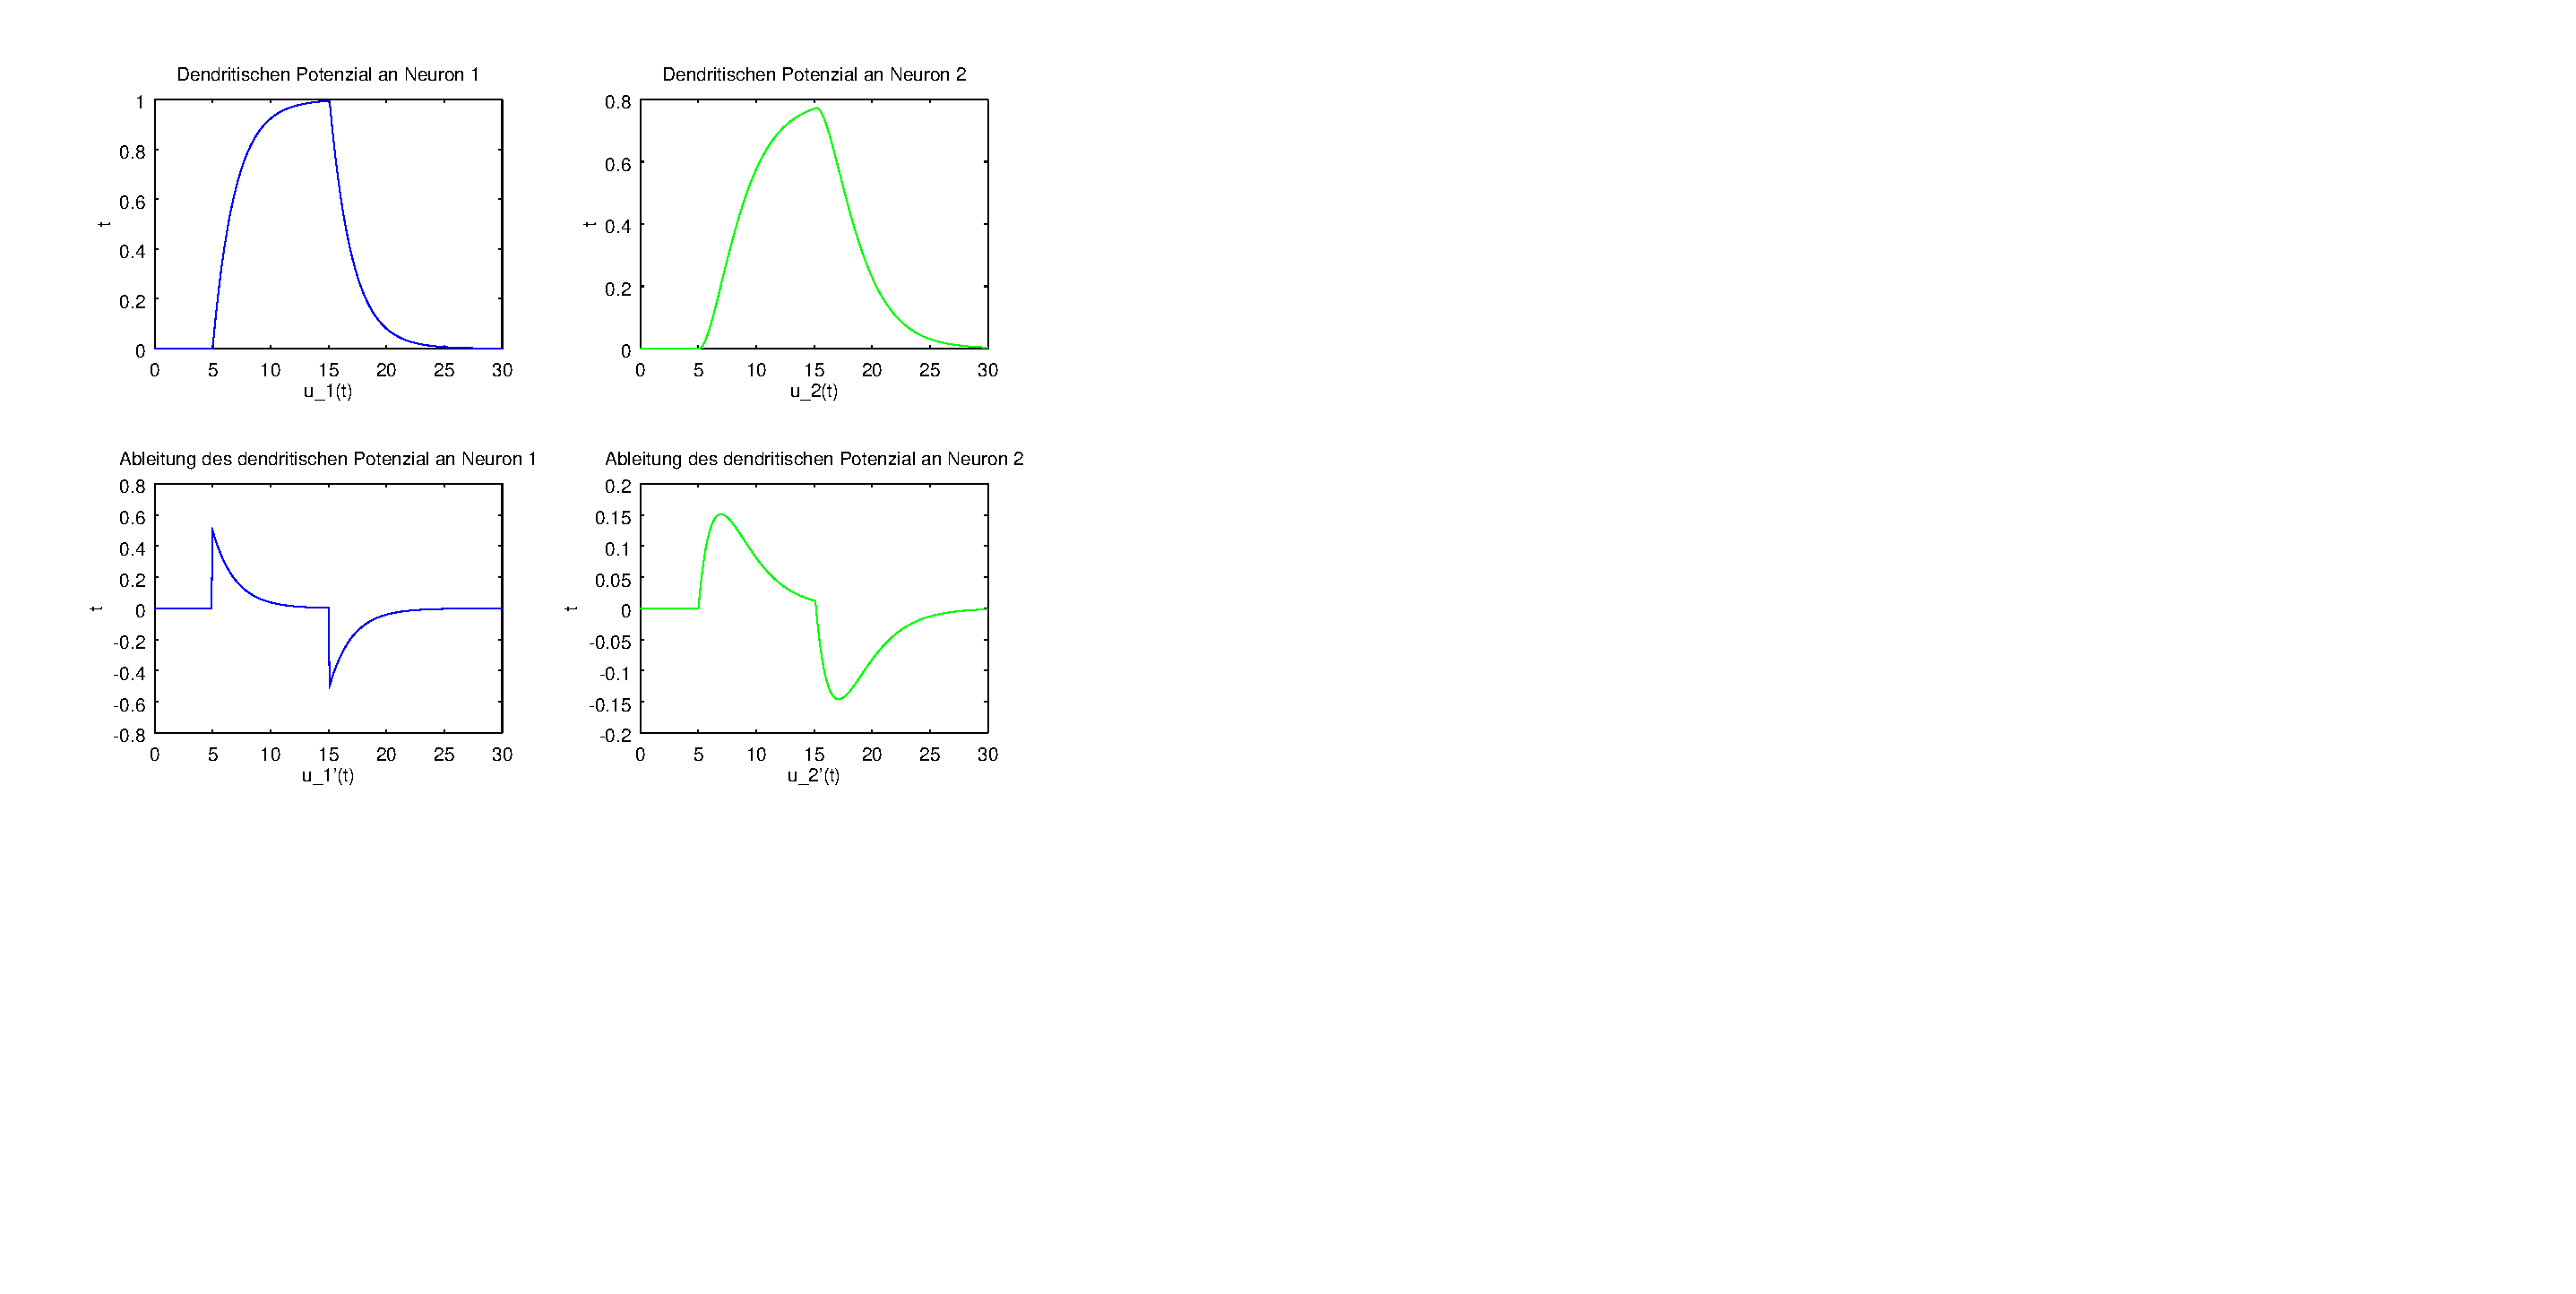
\includegraphics[trim = {0 9cm 27cm 0}, clip,width=\textwidth]{Plot_tau2}
                \caption{Dendritischen Potentiale und deren jeweilige Ableitungen mit $\tau=2$}
            \end{figure} 
        \item           
            Erstes Neuron:
            \begin{eqnarray*}
                0 \cdot \dot{u}_1(t) &=& -u_1(t) + x_1(t) \\
                \Leftrightarrow u_1(t) &=& x_1(t) 
            \end{eqnarray*}
            Zweites Neuron:
            \begin{eqnarray*}
                0 \cdot \dot{u}_2(t) &=& -u_2(t) + 0.8 u_1(t) \\
                u_2(t) &=& 0.8 u_1(t) 
            \end{eqnarray*}
            Für $\tau = 0$ ist die Flankensteigung unendlich hoch und das Eingangssignal wird unverändert vom
            Neuron wieder ausgegeben, beziehungsweise nur skaliert.
    \end{enumerate}

    \subsection{Übertragungszeit}
    Eine Übertragungszeit führt dazu das die Antwort des zweiten Neurons auf das Signal des ersten Neurons verzögert
    wird, das heißt $u_2(t)$ wird nach rechts verschoben.
\end{document}
